\documentclass[12pt]{article}
\pagenumbering{gobble}

\usepackage{amsmath}
\usepackage{amsfonts}
\usepackage{amssymb}
\usepackage{fancyhdr}
\usepackage[headheight=0.25in,margin=1in]{geometry}

\usepackage{tikz}

\newcommand{\parens}[1]{\left( #1 \right)}

\newcommand{\N}{\mathbb{N}}
\newcommand{\Z}{\mathbb{Z}}
\newcommand{\Q}{\mathbb{Q}}
\newcommand{\R}{\mathbb{R}}
\newcommand{\C}{\mathbb{C}}

\newcommand{\solution}{\textbf{Solution:}}
\newcommand{\proof}{\textbf{Proof:}}
\newcommand{\done}{\ensuremath{
    \strut\hfill\blacksquare
}}

\linespread{1.25}

\begin{document}
    \pagestyle{fancy}

    \fancyhead[L]{Computer Networks}
    \fancyhead[C]{Lab 2 - IPv4}
    \fancyhead[R]{Alex Agruso}

    \begin{itemize}
        \item [Step 3.)] Packet retrieved from ``\verb|curl https://alexagruso.dev|'':
        \begin{center}
            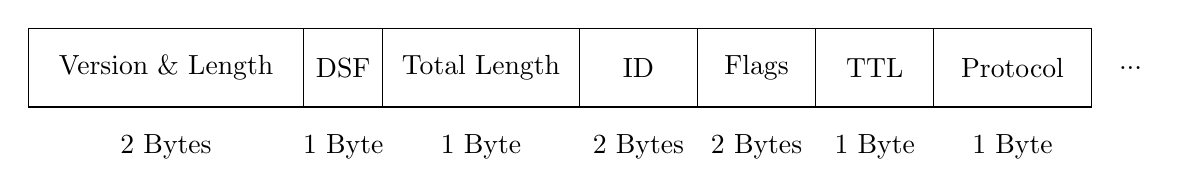
\begin{tikzpicture}
                \draw[] (0,0) rectangle (13.5,1);

                \draw[] (0,0) rectangle (3.5,1)
                node[midway] {Version \& Length};
                \node[] at (1.75,-0.5) {2 Bytes};

                \draw[] (3.5,0) rectangle (4.5,1)
                node[midway] {DSF};
                \node[] at (4,-0.5) {1 Byte};

                \draw[] (4.5,0) rectangle (7,1)
                node[midway] {Total Length};
                \node[] at (5.75,-0.5) {1 Byte};

                \draw[] (7,0) rectangle (8.5,1)
                node[midway] {ID};
                \node[] at (7.75,-0.5) {2 Bytes};

                \draw[] (8.5,0) rectangle (10,1)
                node[midway] {Flags};
                \node[] at (9.25,-0.5) {2 Bytes};

                \draw[] (10,0) rectangle (11.5,1)
                node[midway] {TTL};
                \node[] at (10.75,-0.5) {1 Byte};

                \draw[] (11.5,0) rectangle (13.5,1)
                node[midway] {Protocol};
                \node[] at (12.5,-0.5) {1 Byte};

                \node[] at (14,0.5) {...};
            \end{tikzpicture}
        \end{center}
        \begin{center}
            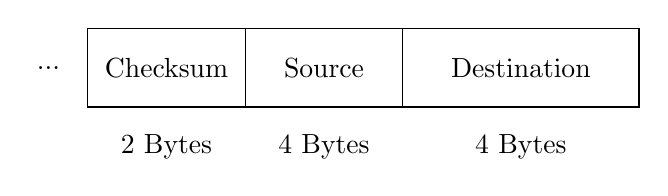
\begin{tikzpicture}
                \node[] at (0.5,-1.5) {...};
                \draw[] (1,-1) rectangle (8,-2);

                \draw[] (1,-1) rectangle (3,-2)
                node[midway] {Checksum};
                \node[] at (2,-2.5) {2 Bytes};

                \draw[] (3,-1) rectangle (5,-2)
                node[midway] {Source};
                \node[] at (4,-2.5) {4 Bytes};

                \draw[] (5,-1) rectangle (8,-2)
                node[midway] {Destination};
                \node[] at (6.5,-2.5) {4 Bytes};
            \end{tikzpicture}
        \end{center}

        \begin{itemize}
            \item [1.)] Based on the packet information, my IP address is
            \verb|153.33.157.22| while the IP address of \verb|alexagruso.dev|
            is \verb|64.23.211.94|.

            \item [2.)] The header length field is explicitly set to 20, while
            the total length field is set to 52, thus we can assume that the
            total length encommpasses both the headers and the payload.

            \item [3.)] While the identifcation differs for each packet, there
            are common prefixes, notably \verb|xe**| and \verb|75**| in my case.
            This is the case in both directions.

            \item [4.)] Each packet with my IP address as it's source has a TTL
            of 52, thus that must be the initial TTL. It is not the maximum
            possible value, as the response packets have a TTL of 64.

            \item [5.)] The flag header of the packet has a value of \verb|0400|,
            and inspecting in wireshark I found that the ``don't fragment'' bit is
            set to 1, thus the packet is not fragmented.

            \item [6.)] In my case, the length of the IP header was 20 bytes, but
            in the data this is encoded as a 5, thus the length is given in words
            (assuming 4 byte words) rather than bytes.
        \end{itemize}

        \item [Step 4.)] \verb| |
        \begin{center}
            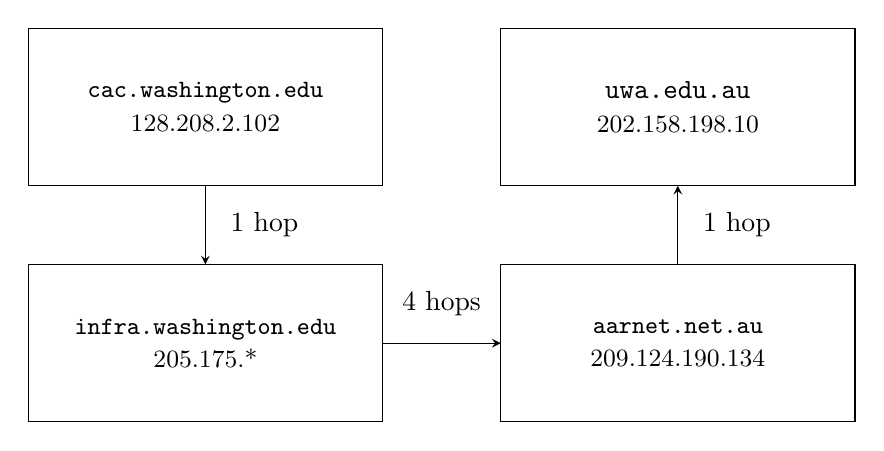
\begin{tikzpicture}
                \draw (0,0) rectangle (4.5,2)
                    node[midway,align=center]
                    {\small\verb|cac.washington.edu| \\ \small128.208.2.102};
                \draw[-stealth] (2.25,0) -- (2.25,-1);
                \node[] at (3,-0.5) {1 hop};

                \draw (0,-1) rectangle (4.5,-3)
                    node[midway,align=center]
                    {\small\verb|infra.washington.edu| \\ \small205.175.*};
                \draw[-stealth] (4.5,-2) -- (6,-2);
                \node[] at (5.25,-1.5) {4 hops};

                \draw (6,-1) rectangle (10.5,-3)
                    node[midway,align=center]
                    {\small\verb|aarnet.net.au| \\ \small209.124.190.134};
                \draw[-stealth] (8.25,-1) -- (8.25,0);
                \node[] at (9,-0.5) {1 hop};

                \draw (6,0) rectangle (10.5,2)
                    node[midway,align=center]
                    {\verb|uwa.edu.au| \\ \small202.158.198.10};
            \end{tikzpicture}
        \end{center}

        \item [Step 5.)] \begin{itemize}
            \item [1.)] Choosing a packet from the remote server and splitting
            it into 2 byte words, we get \verb|4502|, \verb|0120|, \verb|7537|,
            \verb|4000|, \verb|3406|, \verb|d88c|, \verb|4017|, \verb|d35e|,
            \verb|0abf|, and \verb|d9dd|.

            \item [2.)] Summing these words, we get \verb|3fffc|.

            \item [3.)] Taking the 1's complement sum, we add \verb|3| + \verb|fffc|
            to get \verb|10000| then invert the bits, resulting in \verb|ffff|.

            \item [4.)] Because the result is \verb|ffff|, we can conclude that the
            checksum is correct.
        \end{itemize}
    \end{itemize}
\end{document}
